% Drawing 154/08-31 -- folder 154, batch 08, archive page 156 (PDF page 157).
% Transcription: entre parenthèses au crayon, un dessin en couleur, but de la flèche $\sigma_1$ : deux configurations réunies par « ou ». Dans chacune, une droite verte pleine coupe deux paires de droites orange ; elle passe sous le premier croisement à gauche (triangle ombré au crayon) et au-dessus du premier croisement à droite (triangle rempli de brun), et sous le second croisement, dont le triangle est marqué $T$ ; près du premier croisement, une flèche verte repassée à l'encre noire, vers la gauche, marquée $-\omega^{*}$
% Kind: in pencil brackets, two configurations joined by « ou »: solid green line across two orange crossings, arrow to the left marked -omega* (target of sigma_1). Method 2 (schematic redraw from the facsimile). Status: ok.
% Notes: In pencil brackets, at the head of the arrow sigma_1 of the star diagram. Two configurations with « ou » between them. Left: a solid green line passes below the first orange crossing (the triangle between them shaded in pencil) and below the second (T in pencil at its right); under the line, right of the first pair, a thick green arrow pointing left, gone over in black ink (black head and shaft), « -omega* » in pencil below. Right: the line passes above the first crossing (the small triangle between line and crossing filled dark brown) and below the second (T at its right); above the line, right of the first pair, the same green and black arrow pointing left, « -omega* » below the line. 8 orange strokes, 4 crossings, 2 green lines, 2 arrows, labels T, T, -omega* twice, ou. Read from the 400 dpi colour scan; each pair of orange strokes fitted to the ink and drawn through its computed crossing, the triangles bounded by the computed intersections with the green line; the redraw was overlaid on the scan and agrees to within a stroke's width. The felt strokes are drawn straight (slight curvature of a few strokes not reproduced). Redrawn 2026-11-12 (issue 128): to check again.
% Coordinates: 1 unit = 1 mm = 1/100 of the crop width, same scale on both axes (bbox in page fractions: [0.586, 0.305, 0.934, 0.359]).
% Redrawn by Claude (claude-fable-5-2), issue #128, 2026-11-12; not checked by a human; not compiled (no TeX in the session).
% Rights: reproduces part of the work -- behind RENDER_TRANSCRIPTS, never published by itself.
\documentclass[tikz,border=3pt]{standalone}
\usepackage{amsmath,amssymb}
\usetikzlibrary{patterns,arrows.meta}
\tikzset{Or/.style={orange!90!black}, Lg/.style={green!60!black!70}, Br/.style={brown!80!black}, pencil/.style={black!55}, mpt/.style={circle,draw,inner sep=1.3pt}, pt/.style={circle,fill,inner sep=0.9pt}}
\colorlet{Or}{orange!90!black}\colorlet{Lg}{green!60!black!70}\colorlet{Br}{brown!80!black}
\begin{document}
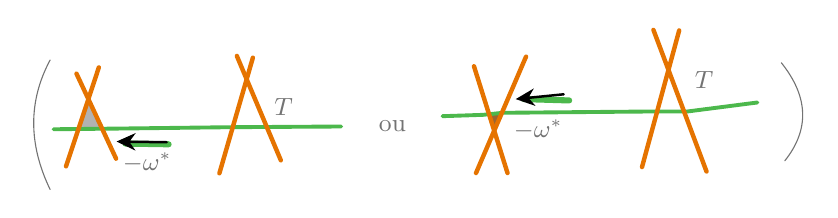
\begin{tikzpicture}[x=1mm,y=1mm,line cap=round,line join=round,font=\scriptsize]
\fill[black!30] (7.9,-10) -- (6.64,-13.79) -- (9.65,-13.76) -- cycle;
\fill[Br] (59.44,-14.01) -- (58.78,-11.92) -- (60.41,-11.75) -- cycle;
\draw[pencil] (3.04,-5.04) .. controls (0.26,-10.23) and (0.26,-15.71) .. (3.04,-21.48);
\draw[pencil] (95.91,-5.39) .. controls (99.36,-9.71) and (99.51,-13.86) .. (96.35,-17.83);
\draw[Lg,line width=1.4pt] (3.48,-13.83) -- (11.91,-13.74) -- (25.74,-13.57) -- (40,-13.48);
\draw[Or,line width=1.6pt] (9.23,-5.97) -- (7.9,-10) -- (5.06,-18.54);
\draw[Or,line width=1.6pt] (6.39,-6.77) -- (7.9,-10) -- (11.42,-17.57);
\draw[Lg,line width=2.2pt] (18.09,-15.74) -- (12.61,-15.65);
\draw[line width=0.9pt,-{Stealth[length=2.4mm,width=2.2mm]}] (17.83,-15.48) -- (11.48,-15.39);
\node[pencil,inner sep=1pt] at (15.39,-18.09) {\small $-\omega^{*}$};
\draw[Or,line width=1.6pt] (28.79,-4.74) -- (28,-7.48) -- (24.54,-19.42);
\draw[Or,line width=1.6pt] (26.75,-4.51) -- (28,-7.48) -- (32.34,-17.77);
\node[pencil,inner sep=1pt] at (32.7,-11.04) {\small $T$};
\node[pencil,inner sep=1pt] at (46.52,-13.48) {\small ou};
\draw[Lg,line width=1.4pt] (52.87,-12.17) -- (58,-12) -- (60.52,-11.74) -- (79.74,-11.57) -- (84,-11.57) -- (92.87,-10.43);
\draw[Or,line width=1.6pt] (56.87,-5.83) -- (59.44,-14.01) -- (61.13,-19.39);
\draw[Or,line width=1.6pt] (63.48,-4.61) -- (59.44,-14.01) -- (57.13,-19.39);
\draw[Lg,line width=2.2pt] (68.96,-10.17) -- (63.22,-10);
\draw[line width=0.9pt,-{Stealth[length=2.4mm,width=2.2mm]}] (68.26,-9.39) -- (62.17,-10);
\node[pencil,inner sep=1pt] at (65.04,-13.91) {\small $-\omega^{*}$};
\draw[Or,line width=1.6pt] (79.66,-1.21) -- (81.57,-6.29) -- (86.4,-19.19);
\draw[Or,line width=1.6pt] (82.93,-1.28) -- (81.57,-6.29) -- (78.21,-18.63);
\node[pencil,inner sep=1pt] at (86.09,-7.57) {\small $T$};
\end{tikzpicture}
\end{document}
